


















































\section{Evaluations}
\subsection{Main Results}
\subsubsection{Evaluation Settings}
\paragraph{Benchmarks}
We evaluate Kimi K2.5 on a comprehensive benchmark suite spanning text-based reasoning, competitive and agentic coding, multimodal understanding (image and video), autonomous agentic execution, and computer use. Our benchmark taxonomy is organized along the following capability axes:
\begin{itemize}
\item \textbf{Reasoning \& General}: Humanity's Last Exam (HLE)~\citep{phan2025humanitysexam}, AIME 2025~\citep{aime2025}, HMMT 2025 (Feb)~\citep{hmmt2025feb}, IMO-AnswerBench~\citep{luong-etal-2025-towards}, GPQA-Diamond~\citep{rein2024gpqa}, MMLU-Pro~\citep{wang2024mmluprorobustchallengingmultitask}, SimpleQA Verified~\citep{haas2025simpleqaverifiedreliablefactuality}, AdvancedIF~\citep{he2025advancedifrubricbasedbenchmarkingreinforcement}, and LongBench v2~\citep{bai2025longbenchv2deeperunderstanding}.
\item \textbf{Coding}: 
SWE-Bench Verified~\citep{jimenez2023swe}, 
SWE-Bench Pro (public)~\citep{deng2025swe}, 
SWE-Bench Multilingual~\citep{jimenez2023swe}, 
Terminal Bench~2.0~\citep{merrill2026terminal}, 
PaperBench (CodeDev)~\citep{starace2025paperbench}, 
CyberGym~\citep{wang2025cybergym}, 
SciCode~\citep{tian2024scicode}, 
OJBench (cpp)~\citep{wang2025ojbench}, 
and LiveCodeBench (v6)~\citep{jain2024livecodebench}.
\item \textbf{Agentic Capabilities}: BrowseComp~\cite{wei2025browsecomp}, WideSearch~\cite{wong2025widesearch},DeepSearchQA~\cite{vedula2025deepsearchqa}, FinSearchComp (T2\&T3)~\cite{hu2025finsearchcomp}, Seal-0~\cite{pham2025sealqa}, GDPVal~\cite{patwardhan2025gdpval}.
\item \textbf{Image Understanding}: \textit{(math \& reasoning)} MMMU-Pro~\citep{yue2025mmmupro}, MMMU (val)~\citep{yue2023mmmu}, CharXiv (RQ)~\citep{wang2024charxiv}, MathVision~\citep{wang2024mathvision} and MathVista (mini)~\citep{lu2024mathvista}; \textit{(vision knowledge)} SimpleVQA~\citep{cheng2025simplevqa} and WorldVQA~\footnote{https://github.com/MoonshotAI/WorldVQA}; \textit{(perception)} ZeroBench (w/ and w/o tools)~\citep{roberts2025zerobench}, BabyVision~\citep{chen2026babyvision}, BLINK~\citep{fu2024blinkmultimodallargelanguage} and MMVP~\citep{tong2024eyeswideshutexploring}; \textit{(OCR \& document)} OCRBench~\citep{liu2024ocrbench}, OmniDocBench~1.5~\citep{ouyang2025omnidocbench} and InfoVQA~\citep{mathew2021infovqa}.
\item \textbf{Video Understanding}: VideoMMMU~\citep{hu2025videommmu}, MMVU~\citep{zhao2025mmvu}, MotionBench~\citep{hong2025motionbench}, Video-MME~\citep{fu2025videomme} (\textit{with subtitles}), LongVideoBench~\citep{wu2024longvideobench}, and LVBench~\citep{wang2025lvbench}.
\item \textbf{Computer Use}:  OSWorld-Verified~\cite{osworld_verified, OSWorld}, and WebArena ~\citep{zhou2023webarena}.
\end{itemize}

\newcolumntype{P}[1]{>{\centering\arraybackslash}p{#1}}
\begin{table}[htbp]
\vspace{-2em} % 上移 1 个行高，可以调整数值
\centering
\footnotesize
\setlength{\tabcolsep}{3pt}

\caption{Performance comparison of Kimi K2.5 against open-source and proprietary models. \textbf{Bold} denotes the global SOTA; Data points marked with * are taken from our internal evaluations. $^{\dagger}$ refers to their scores of text-only subset.}
\label{tab:instruct_eval}

\begin{tabular}{@{}l | P{1.5cm} | P{2cm} P{2cm} P{2cm} | P{2cm} P{2cm}@{}} 
\toprule
& & \multicolumn{3}{c|}{\textbf{Proprietary}} & \multicolumn{2}{c}{\textbf{Open Source}} \\ 
\cmidrule(l{2pt}r{2pt}){3-5} \cmidrule(l{2pt}r{2pt}){6-7}
\textbf{Benchmark} & \textbf{Kimi K2.5} & \textbf{Claude Opus 4.5} & \textbf{GPT-5.2 (xhigh)} & \textbf{Gemini 3 Pro} & \textbf{DeepSeek-V3.2} & \textbf{Qwen3-VL-235B-A22B} \\
\midrule
\multicolumn{7}{@{}l}{\textbf{Reasoning \& General}} \\
HLE-Full & 30.1 & 30.8 & 34.5 & \textbf{37.5} & 25.1$^{\dagger}$ & - \\
HLE-Full~w/ tools & \textbf{50.2 }& 43.2 & 45.5 & 45.8 & 40.8$^{\dagger}$ & - \\
AIME~2025 & 96.1 & 92.8 & \textbf{100} & 95.0 & 93.1 & - \\
HMMT~2025 (Feb) & 95.4 & 92.9* & \textbf{99.4} & 97.3* & 92.5 & - \\
IMO-AnswerBench & 81.8 & 78.5* & \textbf{86.3} & 83.1* & 78.3 & - \\
GPQA-Diamond & 87.6 & 87.0 & \textbf{92.4} & 91.9 & 82.4 & - \\
MMLU-Pro & 87.1 & 89.3* & 86.7* & \textbf{90.1} & 85.0 & - \\
SimpleQA Verified & 36.9 & 44.1 & 38.9 & \textbf{72.1} & 27.5 & - \\
AdvancedIF & 75.6 & 63.1 & \textbf{81.1} & 74.7 & 58.8 & - \\
LongBench v2 & 61.0 & 64.4* & 54.5* & \textbf{68.2*} & 59.8* & - \\
\midrule

\multicolumn{7}{@{}l}{\textbf{Coding}} \\
SWE-Bench Verified & 76.8 & \textbf{80.9} & 80.0 & 76.2 & 73.1 & - \\
SWE-Bench Pro (public) & 50.7 & 55.4* & \textbf{55.6} & - & - & - \\
SWE-Bench Multilingual & 73.0 & \textbf{77.5} & 72.0 & 65.0 & 70.2 & - \\
Terminal Bench~2.0 & 50.8 & \textbf{59.3} & 54.0 & 54.2 & 46.4 & - \\
PaperBench (CodeDev) & 63.5 & \textbf{72.9*} & 63.7* & - & 47.1 & - \\
CyberGym & 41.3 & \textbf{50.6} & - & 39.9* & 17.3* & - \\
SciCode & 48.7 & 49.5 & 52.1 & \textbf{56.1} & 38.9 & - \\
OJBench (cpp) & 57.4 & 54.6* & - & \textbf{68.5*} & 54.7* & - \\
LiveCodeBench (v6) & 85.0 & 82.2* & - & \textbf{87.4*} & 83.3 & - \\
\midrule
\multicolumn{7}{@{}l}{\textbf{Agentic}} \\
BrowseComp & \textbf{60.6} & 37.0 & \multirow{2}{*}{65.8} & 37.8 & 51.4 & - \\
BrowseComp~(w/ ctx manage) & \textbf{74.9} & 57.8 & & 59.2 & 67.6 & - \\
BrowseComp~(Agent Swarm) & \textbf{78.4} & - & - & - & - & - \\
WideSearch & 72.7 & \textbf{76.2*} & - & 57.0 & 32.5* & - \\
WideSearch~(Agent Swarm) & \textbf{79.0} & - & - & - & - & - \\
DeepSearchQA & \textbf{77.1} & 76.1* & 71.3* & 63.2* & 60.9* & - \\
FinSearchCompT2\&T3 & \textbf{67.8} & 66.2* & - & 49.9 & 59.1* & - \\
Seal-0 & \textbf{57.4} & 47.7* & 45.0 & 45.5* & 49.5* & - \\
GDPVal-AA & 41.0 & 45.0 & \textbf{48.0} & 35.0 & 34.0 & - \\

\midrule
\multicolumn{7}{@{}l}{\textbf{Image}} \\
MMMU-Pro & 78.5 & 74.0 & 79.5* & \textbf{81.0} & - & 69.3 \\
MMMU (val) & 84.3 & 80.7 & 86.7* & \textbf{87.5*} & - & 80.6 \\
CharXiv (RQ) & 77.5 & 67.2* & \textbf{82.1} & 81.4 & - & 66.1 \\
MathVision & 84.2 & 77.1* & 83.0 & \textbf{86.1*} & - & 74.6 \\
MathVista (mini) & \textbf{90.1} & 80.2* & 82.8* & 89.8* & - & 85.8 \\
SimpleVQA & \textbf{71.2} & 69.7* & 55.8* & 69.7* & - & 56.8* \\
WorldVQA & 46.3 & 36.8 & 28.0 & \textbf{47.4} & - & 23.5 \\
ZeroBench & \textbf{9} & 3* & \textbf{9*} & 8* & - & 4* \\
ZeroBench~w/ tools & 11 & 9* & 7* & \textbf{12*} & - & 3* \\
BabyVision & 36.5 & 14.2 & 34.4 & \textbf{49.7} & - & 22.2 \\
BLINK & \textbf{78.9}  & 68.8* & -  & 78.7* & - & 68.9 \\
MMVP & 87.0 & 80.0* & 83.0* & \textbf{90.0*} & - & 84.3 \\
OmniDocBench~1.5 & \textbf{88.8} & 87.7* & 85.7 & 88.5 & - & 82.0* \\
OCRBench & \textbf{92.3} & 86.5* & 80.7* & 90.3* & - & 87.5 \\
InfoVQA (test) & \textbf{92.6} & 76.9* & 84* & 57.2* & - & 89.5 \\


\midrule
\multicolumn{7}{@{}l}{\textbf{Video}} \\
VideoMMMU & 86.6 & 84.4* & 85.9 & \textbf{87.6} & - & 80.0 \\
MMVU & 80.4 & 77.3* & \textbf{80.8*} & 77.5* & - & 71.1 \\
MotionBench & \textbf{70.4} & 60.3* & 64.8* & 70.3 & - & - \\
Video-MME & 87.4 & 77.6* & 86.0* & \textbf{88.4*} & - & 79.0 \\
LongVideoBench & \textbf{79.8} & 67.2* & 76.5* & 77.7* & - & 65.6* \\
LVBench & \textbf{75.9} & 57.3 & - & 73.5* & - & 63.6 \\
\midrule

\multicolumn{7}{@{}l}{\textbf{Computer Use}} \\

OSWorld-Verified &  63.3 &  \textbf{66.3}& 8.6* & 20.7* & - & 38.1 \\
WebArena &  58.9 & \textbf{63.4}* & - & - & - & 26.4* \\

\bottomrule
\end{tabular}
\end{table}



\begin{table}[htbp]
\centering
\hspace{0.3cm}
\caption{Performance and token efficiency of some reasoning models. Average output token counts (in thousands) are shown in parentheses.}
\begin{tabular}{cc|ccc}
\toprule
\textbf{Benchmark} & \textbf{Kimi K2.5} & \textbf{Kimi K2} & \textbf{Gemini-3.0} & \textbf{DeepSeek-V3.2} \\
 &  & \textbf{Thinking} & \textbf{Pro} & \textbf{Thinking} \\
\midrule
AIME 2025 & 96.1 (25k) & 94.5 (30k) & 95.0 (15k) & 93.1 (16k) \\
HMMT Feb 2025 & 95.4 (27k) & 89.4 (35k) & 97.3 (16k) & 92.5 (19k) \\
HMMT Nov 2025 & 91.1 (24k) & 89.2 (32k) & 94.5 (15k) & 90.2 (18k) \\
IMO-AnswerBench & 81.8 (36k) & 78.6 (37k) & 83.1 (18k) & 78.3 (27k) \\
LiveCodeBench & 85.0 (18k) & 82.6 (25k) & 87.4 (13k) & 83.3 (16k) \\
GPQA Diamond & 87.6 (14k) & 84.5 (13k) & 91.9 (8k) & 82.4 (7k) \\
HLE-Text  & 31.5 (24k) & 23.9 (29k) & 38.4 (13k) & 25.1 (21k) \\
\bottomrule
\end{tabular}
\label{tab:k2.5-te}
\end{table}

\paragraph{Baselines}
We benchmark against state-of-the-art proprietary and open-source models. For proprietary models, we compare against Claude Opus 4.5 (with extended thinking) \citep{opus45report}, GPT-5.2 (with xhigh reasoning effort) \citep{gpt52report}, and Gemini 3 Pro (with high reasoning-level) \citep{gemini3pro}. For open-source models, we include DeepSeek-V3.2 (with thinking mode enabled)~\citep{deepseekai2025deepseekv32pushingfrontieropen} for text benchmarks, while vision benchmarks report Qwen3-VL-235B-A22B-Thinking~\citep{bai2025qwen3vltechnicalreport} instead.

\paragraph{Evaluation Configurations}
Unless otherwise specified, all Kimi K2.5 evaluations use temperature = 1.0, top-p = 0.95, and a context length of 256k tokens. Benchmarks without publicly available scores were re-evaluated under identical conditions and marked with an asterisk (*). The full evaluation settings can be found in appendix~\ref{app:eval_details}.

\subsubsection{Evaluation Results}
\label{sec:eval_results}
Comprehensive results comparing Kimi K2.5 against proprietary and open-source baselines are presented in Table~\ref{tab:instruct_eval}. We highlight key observations across core capability domains:
\paragraph{Reasoning and General}
Kimi K2.5 achieves competitive performance with top-tier proprietary models on rigorous STEM benchmarks. On Math tasks, AIME 2025, K2.5 scores 96.1\%, approaching GPT-5.2's perfect score while outperforming Claude Opus 4.5 (92.8\%) and Gemini 3 Pro (95.0\%). This high-level performance extends to the HMMT 2025 (95.4\%) and IMO-AnswerBench (81.8\%), demonstrating K2.5's superior reasoning depth. Kimi K2.5 also exhibits remarkable knowledge and scientific reasoning capabilities, scoring 36.9\% on SimpleQA Verified, 87.1\% on MMLU-Pro and 87.6\% on GPQA. Notably, on HLE without the use of tools, K2.5 achieves an HLE-Full score of 30.1\%, with component-wise scores of 31.5\% on text subset and 21.3\% on image subset. When tool-use is enabled, K2.5’s HLE-Full score rises to 50.2\%, with 51.8\% (text) and 39.8\% (image), significantly outperforming Gemini 3 Pro (45.8\%) and GPT-5.2 (45.5\%). In addition to reasoning and knowledge, K2.5 shows strong instruction-following performance (75.6\% on AdvancedIF) and competitive long-context abilities, achieving 61.0\% on LongBench v2 compared to both proprietary and open-source models.

\paragraph{Complex Coding and Software Engineering}
Kimi K2.5 exhibits strong software engineering capabilities, especially on realistic coding and maintenance tasks. It achieves 76.8\% on SWE-Bench Verified and 73.0\% on SWE-Bench Multilingual, outperforming Gemini 3 Pro while remaining competitive with Claude Opus 4.5 and GPT‑5.2. On LiveCodeBench v6, Kimi K2.5 reaches 85.0\%, surpassing DeepSeek‑V3.2 (83.3\%) and Claude Opus 4.5 (82.2\%), highlighting its robustness on live, continuously updated coding challenges. On TerminalBench 2.0, PaperBench, and SciCode, it scores 50.8\%, 63.5\%, and 48.7\% respectively, demonstrating stable competition‑level performance in automated software engineering and problem solving across diverse domains. In addition, K2.5 attains a score of 41.3 on CyberGym, on the task of finding previously discovered vulnerabilities in real open‑source software projects given only a high‑level description of the weakness, further underscoring its effectiveness in security‑oriented software analysis.

\paragraph{Agentic Capabilities}
Kimi K2.5 establishes new state-of-the-art performance on complex agentic search and browsing tasks. On BrowseComp, K2.5 achieves 60.6\% without context management techniques, 74.9\% with Discard-all context management \citep{deepseekai2025deepseekv32pushingfrontieropen} — substantially outperforming GPT-5.2's reported 65.8\%, Claude Opus 4.5 (37.0\%) and Gemini 3 Pro (37.8\%). Similarly, WideSearch reaches 72.7\% on item-f1. On DeepSearchQA (77.1\%), FinSearchCompT2\&T3 (67.8\%) and Seal-0 (57.4\%), K2.5 leads all evaluated models, demonstrating superior capacity for agentic deep research, information synthesis, and multi-step tool orchestration.


\paragraph{Vision Reasoning, Knowledge and Perception} Kimi K2.5 demonstrates strong visual reasoning and world knowledge capabilities. It scores 78.5\% on MMMU-Pro, spanning multi-disciplinary multimodal tasks. For world knowledge question answering, K2.5 achieves 71.2\% on SimpleVQA and 46.3\% on WorldVQA. For visual reasoning, it achieves 84.2\% on MathVision, 90.1\% on MathVista (mini), and 36.5\% on BabyVision. For OCR and document understanding, K2.5 delivers outstanding results with 77.5\% on CharXiv (RQ), 92.3\% on OCRBench, 88.8\% on OmniDocBench 1.5, and 92.6\% on InfoVQA (test). On the challenging ZeroBench, Kimi K2.5 achieves 9\% and 11\% with tool augmentation, substantially ahead of competing models. On basic visual perception benchmarks BLINK (78.9\%) and MMVP (87.0\%), we also observe competitive performance of Kimi K2.5, demonstrating its robust real-world visual perceptions.

\paragraph{Video Understanding} Kimi K2.5 achieves state-of-the-art performance across diverse video understanding tasks. It attains 86.6\% on VideoMMMU and 80.4\% on MMVU, rivaling frontier leaderships. With the context-compression and dense temporal understanding abilities of MoonViT-3D, Kimi K2.5 also establishes new global SOTA records in long-video comprehension with 75.9\% on LVBench and 79.8\% on LongVideoBench by feeding over 2,000 frames, while demonstrating robust dense-motion understanding at 70.4\% on the highly-dimensional MotionBench.



\paragraph{Computer-Use Capability} Kimi K2.5 demonstrates state-of-the-art computer-use capability on real-world tasks. On the computer-use benchmark OSWorld-Verified~\citep{osworld_verified,OSWorld}, it achieves a 63.3\% success rate relying solely on GUI actions without external tools. This substantially outperforms open-source models such as Qwen3-VL-235B-A22B (38.1\%) and OpenAI’s computer-use agent framework Operator (o3-based) (42.9\%), while remaining competitive with the current leading CUA model, Claude Opus 4.5 (66.3\%). On WebArena~\citep{zhou2023webarena}, an established benchmark for GUI-based web browsing, Kimi K2.5 achieves a 58.9\% success rate, surpassing OpenAI's Operator (58.1\%) and approaching the performance of Claude Opus 4.5 (63.4\%).
\subsection{Agent Swarm Results}
\label{sec:agent_swarm_results}

\paragraph{Benchmarks}
To rigorously evaluate the effectiveness of the agent swarm framework, we select three representative benchmarks that collectively cover deep reasoning, large-scale retrieval, and real-world complexity:

\begin{itemize}
\item \textbf{BrowseComp}: A challenging deep-research benchmark that requires multi-step reasoning and complex information synthesis.

\item \textbf{WideSearch}: A benchmark designed to evaluate the ability to perform broad, multi-step information seeking and reasoning across diverse sources.

\item \textbf{In-house Swarm Bench}: An internally developed Swarm benchmark, designed to evaluate the agent swarm performance under real-world, high-complexity conditions. It covers four domains: \textit{WildSearch} (unconstrained, real-world information retrieval over the open web), \textit{Batch Download} (large-scale acquisition of diverse resources), \textit{WideRead} (large-scale document comprehension involving more than 100 input documents), and \textit{Long-Form Writing} (coherent generation of extensive content exceeding 100k words). This benchmark incorporates extreme-scale scenarios that stress-test the orchestration, scalability, and coordination capabilities of agent-based systems.
\end{itemize}

\begin{table}[t]
\centering
\footnotesize
\setlength{\tabcolsep}{6pt}
\hspace{0.5cm}
\caption{Performance comparison of Kimi K2.5 Agent Swarm against single-agent and proprietary baselines on agentic search benchmarks. \textbf{Bold} denotes the best result per benchmark.}
\label{tab:agent_swarm_results}
\begin{tabular}{@{}wc{4cm} wc{2cm} wc{2cm}wc{2cm}wc{2cm}wc{2cm}@{}} 
\toprule
\textbf{Benchmark} & \textbf{K2.5 Agent Swarm} & \textbf{Kimi K2.5} & \textbf{Claude Opus 4.5} & \textbf{GPT-5.2} & \textbf{GPT-5.2 Pro} \\
\midrule
BrowseComp & \textbf{78.4} & 60.6 & 37.0 & 65.8 & 77.9 \\
WideSearch & \textbf{79.0} & 72.7 & 76.2 & - & - \\
In-house Swarm Bench & \textbf{58.3} & 41.6 & 45.8 & - & - \\
\bottomrule
\end{tabular}
\end{table}
\paragraph{Performance} Table~\ref{tab:agent_swarm_results} presents the performance of Kimi K2.5 Agent Swarm against single-agent configurations and proprietary baselines. The results demonstrate substantial performance improvements from multi-agent orchestration. On BrowseComp, Agent Swarm achieves 78.4\%, representing a 17.8\% absolute gain over the single-agent K2.5 (60.6\%) and surpassing even GPT-5.2 Pro (77.9\%). Similarly, WideSearch sees a 6.3\% improvement (72.7\% $\to$ 79.0\%) on Item-F1, enabling K2.5 Agent Swarm to outperform Claude Opus 4.5 (76.2\%) and establish a new state-of-the-art. The gains are most pronounced on In-house Swarm bench (16.7\%), where tasks are explicitly designed to reward parallel decomposition. These consistent improvements across benchmarks validate that Agent Swarm effectively converts computational parallelism into qualitative capability gains, particularly for problems requiring broad exploration, multi-source verification, or simultaneous handling of independent sub-tasks.
\begin{figure}[t]
    \centering
    \begin{minipage}[t]{0.48\linewidth}
        \centering
        
\includegraphics[width=0.95\linewidth, keepaspectratio]{figures/agent_swarm_subagents.pdf}
        \caption{The word cloud visualizes heterogeneous K2.5-based sub-agents dynamically instantiated by the Orchestrator across tests.}
        \label{fig:subagent_in_agent_swarm}
    \end{minipage}
    \hfill
    \begin{minipage}[t]{0.48\linewidth}
        \centering
        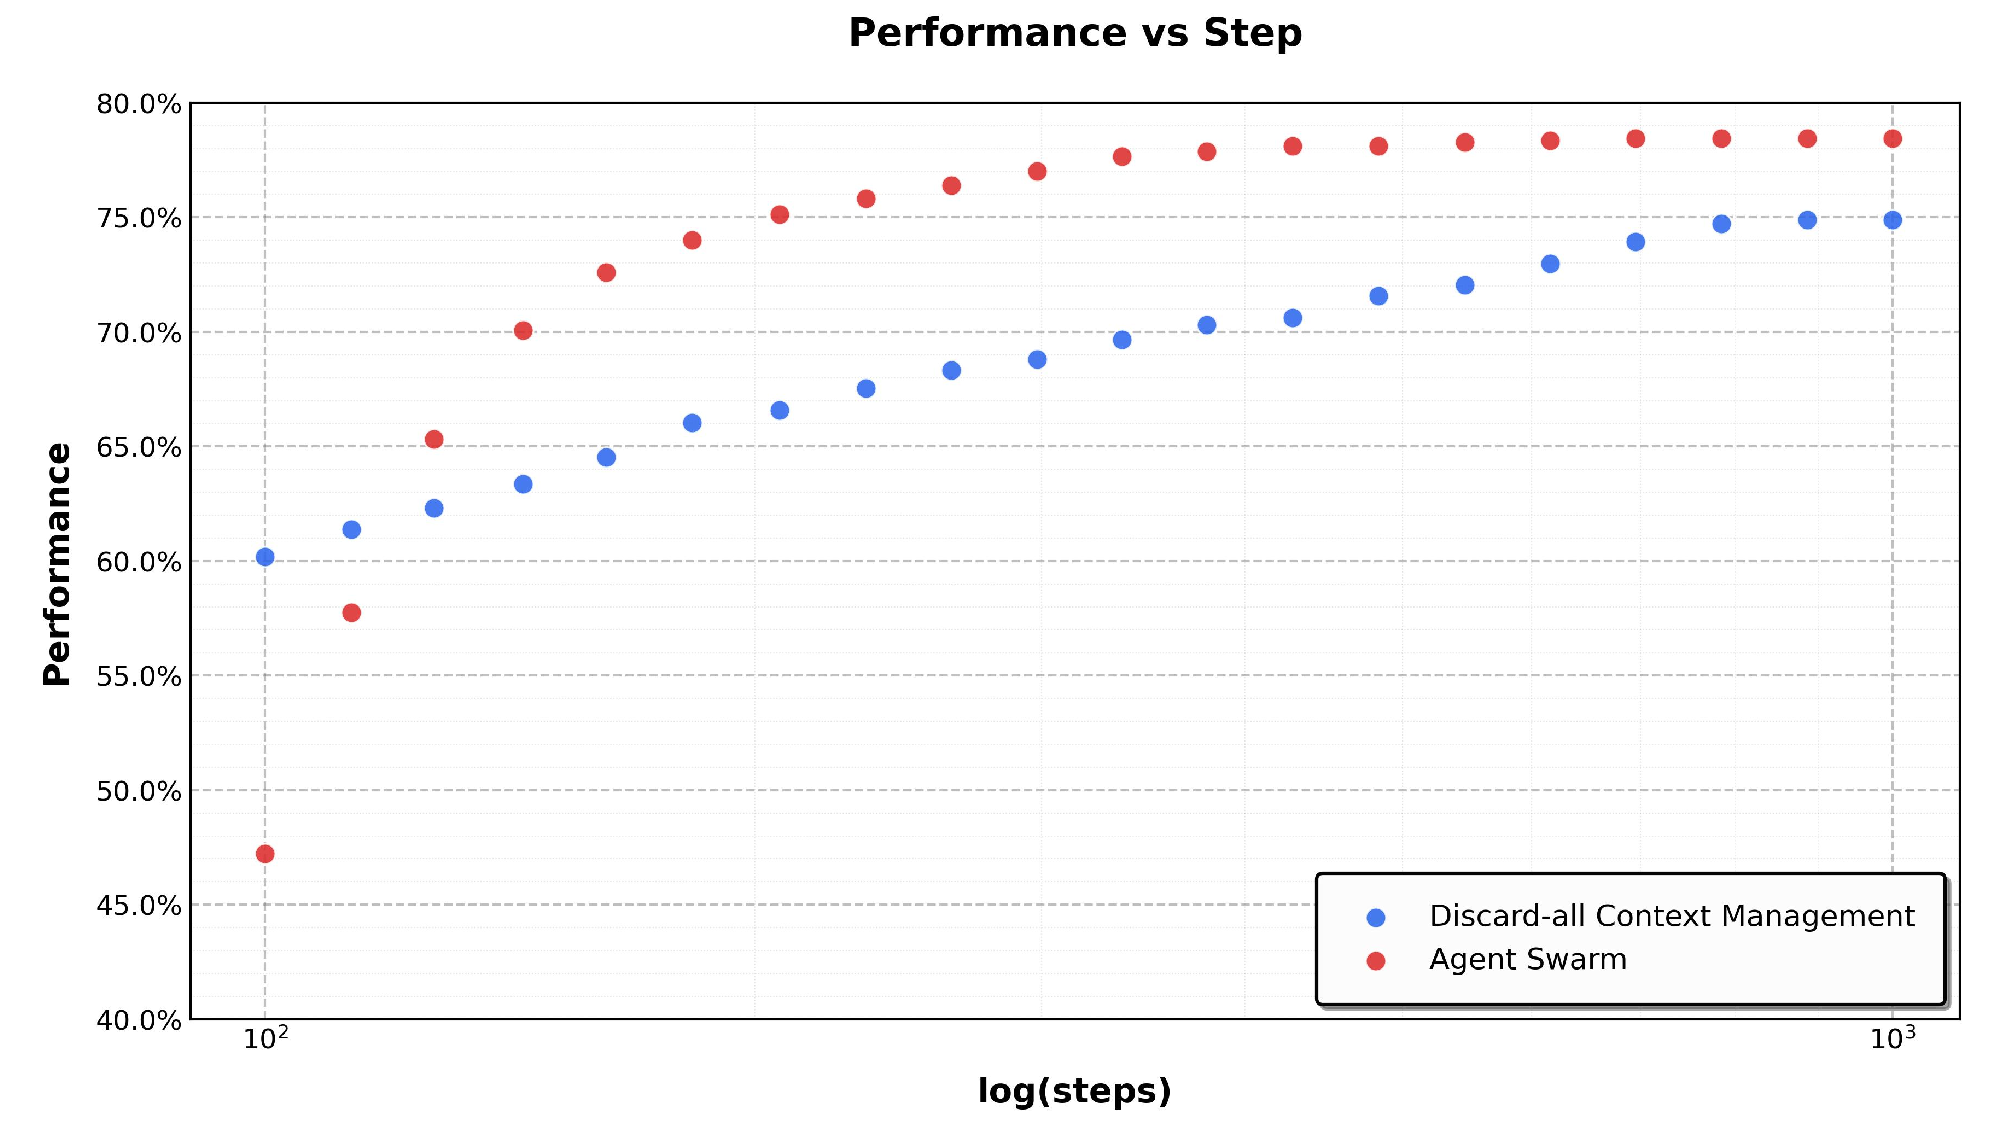
\includegraphics[width=0.95\linewidth, keepaspectratio]{figures/agent_swarm_ctx_mgm.pdf}
        \caption{Comparison of Kimi K2.5 performance under Agent Swarm and Discard-all context management in BrowseComp.}
        \label{fig:agent_swarm_as_ctx_mgm}
    \end{minipage}
\end{figure}

\begin{figure}[t]
    \centering
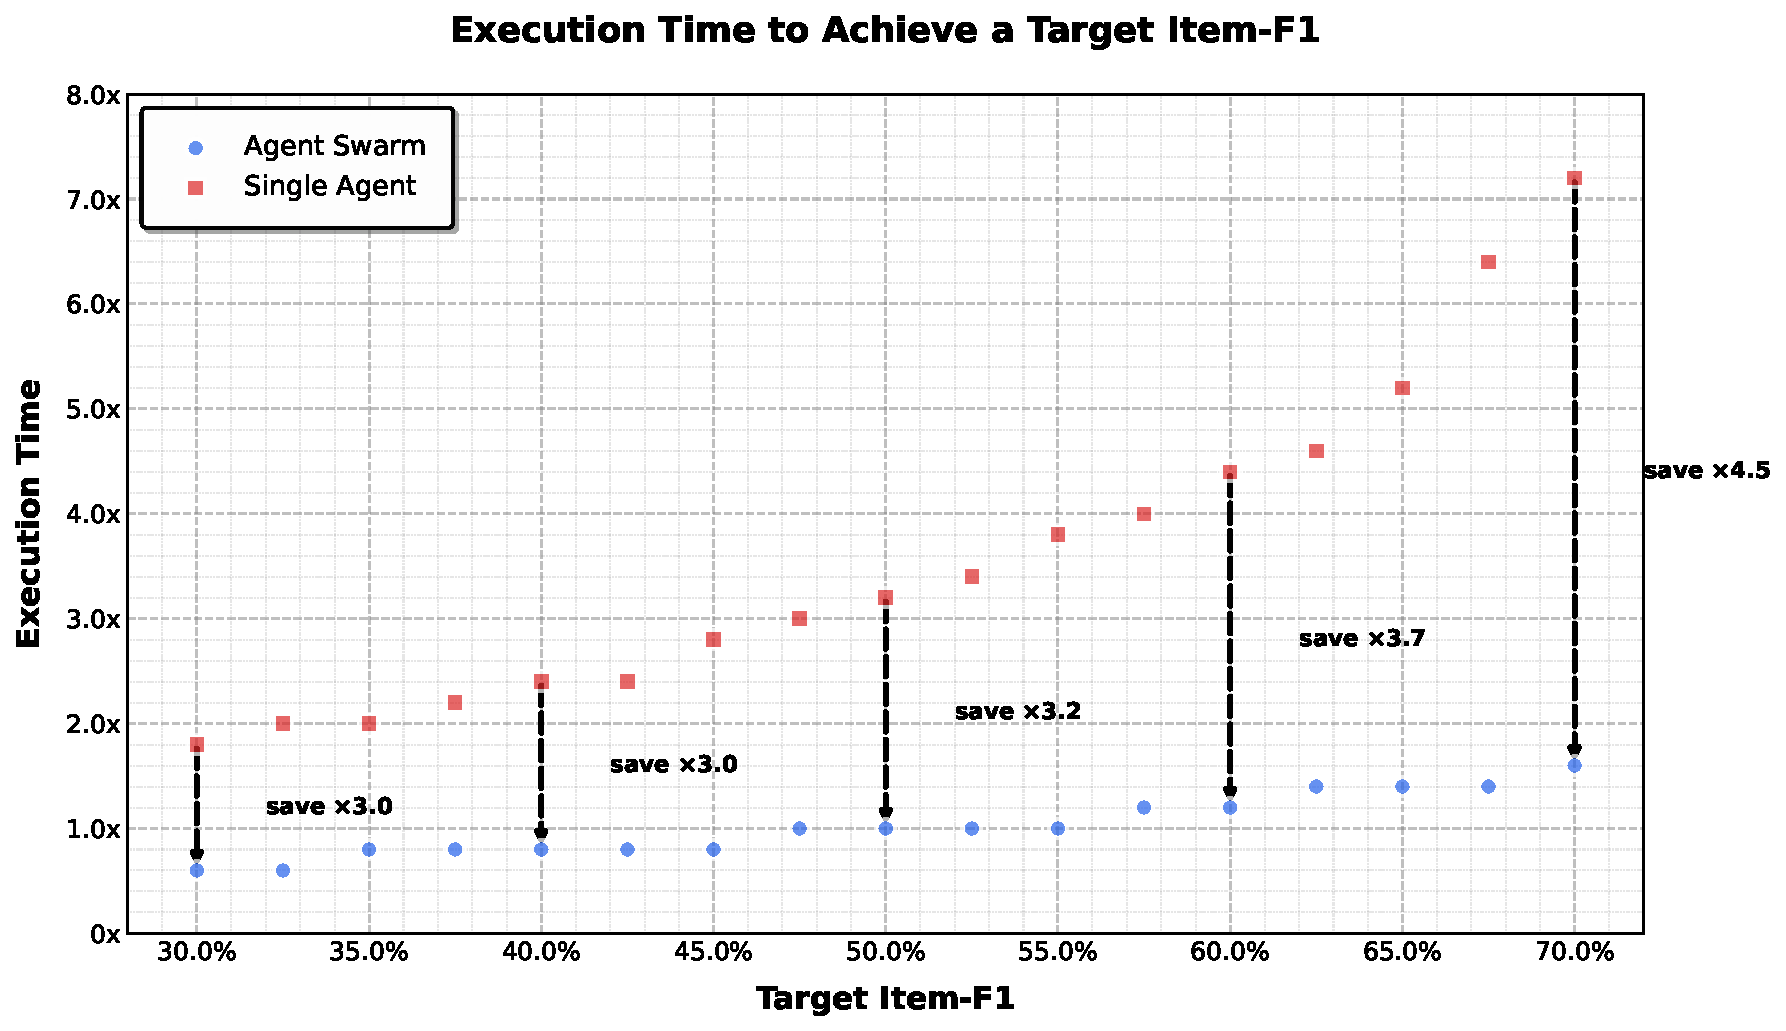
\includegraphics[width=0.618\linewidth, keepaspectratio]{figures/agent_swarm_efficiency.pdf}
    \caption{Agent Swarm achieves 3$\times$--4.5$\times$ faster execution time compared to single-agent baselines as target Item-F1 increases from 30\% to 70\% in WideSearch testing.}
    \label{fig:agent_swarm_efficiency}
\end{figure}

\paragraph{Execution Time Savings via Parallelism} Beyond improved task performance, Agent Swarm achieves substantial wall-clock time reductions through parallel subagent execution. On the WideSearch benchmark, it reduces the execution time required to reach target performance by 3$\times \sim$ 4.5$\times$ compared to a single-agent baseline. As shown in Figure~\ref{fig:agent_swarm_efficiency}, this efficiency gain scales with task complexity: as the target Item-F1 increases from 30\% to 70\%, the single agent's execution time grows from approximately 1.8$\times$ to over 7.0$\times$ the baseline, whereas Agent Swarm maintains near-constant low latency in the range of $0.6\times \sim 1.6\times$. These results indicate that Agent Swarm effectively transforms sequential tool invocations into parallel operations, preventing the linear growth in completion time typically observed as task difficulty increases.

\paragraph{Dynamic Subagent Creation and Scheduling} Within an agent swarm, subagents are dynamically instantiated rather than
pre-defined. Through PARL, the orchestrator learns adaptive policies to create and
schedule self-hosted subagents in response to evolving task structures
and problem states. Unlike static decomposition approaches, this learned policy enables the Orchestrator to reason about the requisite number, timing, and specialization of subagents based on query. Consequently, a heterogeneous agent group emerges organically from this adaptive allocation strategy (Figure~\ref{fig:subagent_in_agent_swarm}).

\paragraph{Agent Swarm as Proactive Context Management} Beyond better performance and runtime acceleration, an agent swarm is a kind of proactive and intelligent context management enabled by multi-agent architecture \citep{anthropicbuildmultiagent}. This approach differs from test-time context truncation strategies such as Hide-Tool-Result \citep{moonshotai2025kimiresearcher}, Summary \citep{wu2025resumunlockinglonghorizonsearch}, or Discard-all \citep{deepseekai2025deepseekv32pushingfrontieropen}, which react to context overflow by compressing or discarding accumulated histories. While effective at reducing token usage, these methods are inherently reactive and often sacrifice structural information or intermediate reasoning.

In contrast, Agent Swarm enables proactive context control through explicit orchestration. Long-horizon tasks are decomposed into parallel, semantically isolated subtasks, each executed by a specialized subagent with a bounded local context. Crucially, these subagents maintain independent working memories and perform local reasoning without directly mutating or contaminating the global context of the central orchestrator. Only task-relevant outputs—rather than full interaction traces—are selectively routed back to the orchestrator. This design induces context sharding rather than context truncation, allowing the system to scale effective context length along an additional architectural dimension while preserving modularity, information locality, and reasoning integrity.

As shown in Figure~\ref{fig:agent_swarm_as_ctx_mgm}, this proactive strategy outperforms Discard-all in both efficiency and accuracy on BrowseComp. By preserving task-level coherence at the orchestrator level while keeping subagent contexts tightly bounded, Agent Swarm enables parallel execution with selective context persistence, retaining only high-level coordination signals or essential intermediate results. Consequently, Agent Swarm operates as an active, structured context manager, achieving higher accuracy with substantially fewer critical steps than uniform context truncation.